\chapter{Current experimental status}
Among the many embodiments of qubits that already exist nowadays, one of the most promising uses the nuclear spin of Phosphorus donors in Silicon. The blueprint for building this kind of qubits was proposed by Bruce Kane back in the 1988.~\cite{Kane1988} Since our proposal is somewhat inspired in that of Kane, we review the basics in the following sections.

% In Solid State Physics there are already some implementation of qubits using Phosphorus donors in Silicon, dopands/vacancies in diamond or even Isotopes of Silicon.

% In the next section we propose a system that can be studied as a candidate for scalable quantum computer.

\section{Kane Proposal}
In 1998 Bruce E. Kane proposed the realization of a quantum computer~\cite{Kane1988} using as qubits the nuclear spin of $^{31}P$ dopants in Silicon (Si:$^{31}$P).
The electronic spin surrounding this nuclear spin would be used to interact with the nuclear spin by tuning its orbital shape with electric gates.

Without much detail, it is expected that the hyperfine interaction could be tuned using an electric gate, $A$, to modify the spatial distribution of the electronic state close to the nucleus of the $^{31}P$, as depicted in figure~\ref{kane}
%~~~~~~~~~~~~~~~~~~~~~~~~~~ FIGURE ~~~~~~~~~~~~~~~~~~~~~~~~~%
\begin{figure}[h!]
\centering
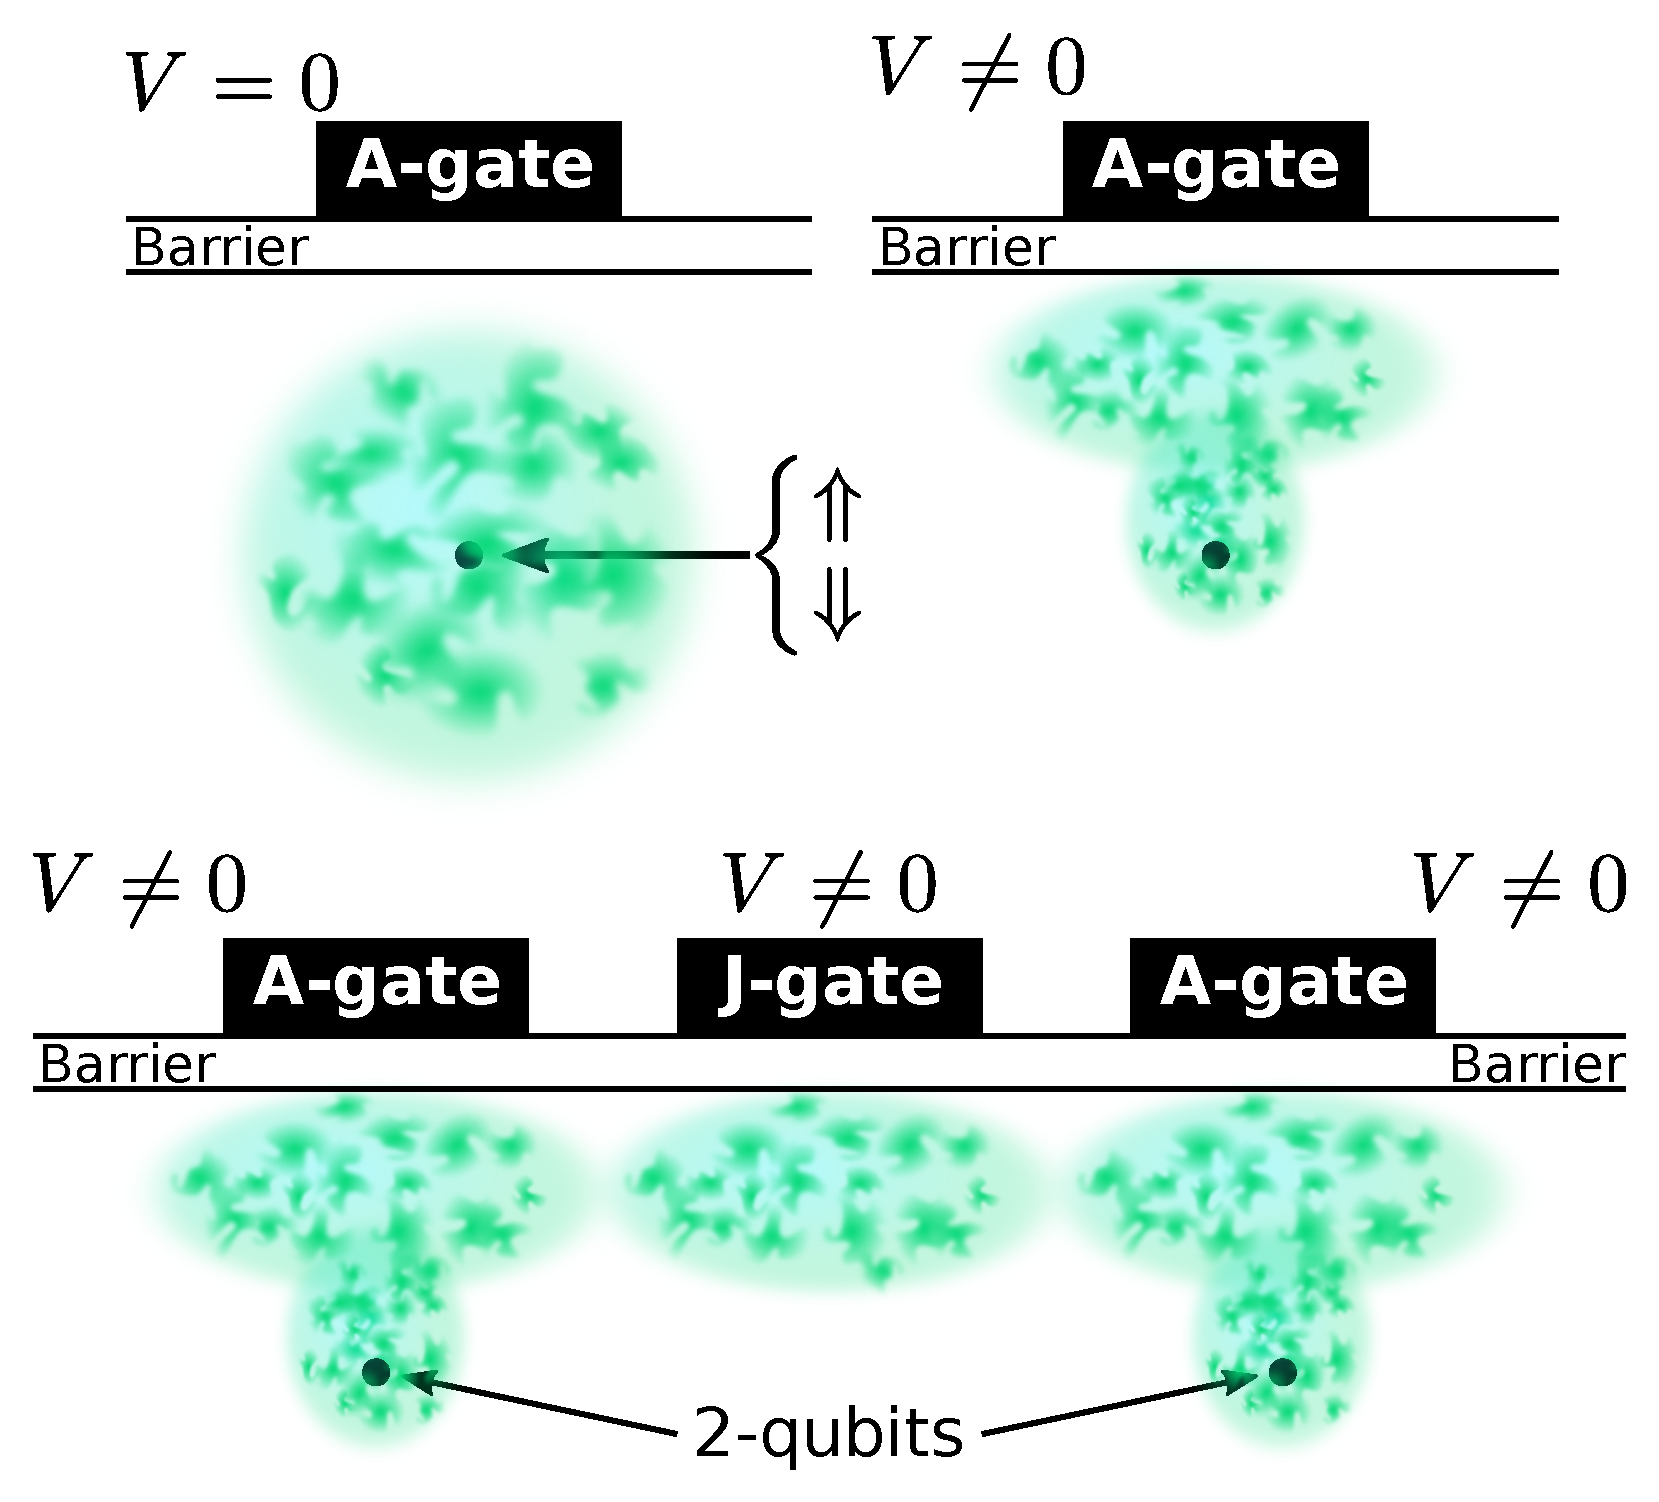
\includegraphics{chapter03/figures/kane.pdf}
\vspace{-5pt}
\caption{Artistic depiction of the Kane proposal for a quantum computer. The single qubit operations would be performed modifying the electronic spin and tuning the hyperfine coupling (with an electric gate $A$) to interact with the nuclear spin. The two qubit operations would be performed by an electronic mediated state controlled also with an intermediate electric gate $J$.}
\label{kane}
\end{figure}
\FloatBarrier
%~~~~~~~~~~~~~~~~~~~~~~~~~~~~~~~~~~~~~~~~~~~~~~~~~~~~~~~~~~~%
Similarly for two qubits to interact with each other Kane proposed an intermediate gate $J$ to aid the process by increasing (decreasing) the electronic density in between the two qubits.

% XXX [graph for Hyperfine and exchange?]

\section{Morello's Implementation}
Kane proposal has been widely pursued and impressive advances have been achieved
\red{Comment on the feasibility of this approach. Electron as another qubit? 2-Qubit operations}


\section{The Graphene analogue}
In hydrogenated graphene we have very similar objects. The Hydrogen has a single nuclear spin, the proton, and the electronic states around it would provide the other spin.

The electronic properties of graphene are highly tunable what suggest that maybe the interactions are tunable as well.

Also the $C$ atoms provide almost no nuclear spins (the abundance of $^{12}C$ is about $98.9\%$ while $^{13}C$ is about $1.1\%$ and only negligible traces of other isotopes~\cite{iupac}), so long relaxation times for the nuclear spin is to be expected


\red{Explain here the similarities and general idea. Possible advantages and drawbacks.}
\red{Motivation for studying graphene and hydrogenated graphene.}


\section{The 1-Qubit Hamiltonian}
The description for the Kane's qubits proposal is that of a nuclear and an electronic spin in an external magnetic and electric field provided by the gates $\mathcal{A}$ and $J$. We will analyze now the properties of such a system.

\subsection{The Zeeman Effect}
The Hamiltonian for a particle with magnetic moment $\vec{m}$ in an external magnetic field $\vec{B}$ is described by the so-called Zeeman term:
\begin{equation}
  H_{\text{Zee}} = -\vec{m}\vec{B}
\end{equation}
The magnetic moment for a particle with mass $m$ and charge $q$ is defined as:
\begin{equation*}
  \vec{m} = g\frac{q}{2m}\vec{S} \qquad\text{with}\qquad \vec{S} =
  \frac{\hbar}{2}\vec{\sigma}
\end{equation*}
Where, renaming $\mu = \frac{q\hbar}{2m}$, we can express the magnetic moment as:
\begin{equation}
  \vec{m} = g\mu\frac{1}{2}\vec{\sigma}
\label{magmom}
\end{equation}
where $g$ is the so-called g-factor\footnote{The g-factor is a dimensionless parameter that for the electron and proton take respectively the values: $g_e=-2.0023\dots$ and $g_p=5.5857\dots$} and $\vec{\sigma}$ is a vector with the Pauli matrices as components $\vec{\sigma}= \left(\sigma_x,\sigma_y,\sigma_z\right)$
\begin{equation}
  \sigma_x=\left(\begin{array}{cc}
    0 & 1 \\
    1 & 0
    \end{array}\right)\quad;\quad
  \sigma_y=\left(\begin{array}{cc}
    0 & -i \\
    i & 0
    \end{array}\right)\quad;\quad
  \sigma_x=\left(\begin{array}{cc}
    1 & 0 \\
    0 & -1
    \end{array}\right)
\end{equation}
The Zeeman term, then, can be rewritten as:
\begin{equation}
  H_{\text{Zee}} = -\vec{m}\vec{B} = -g\mu\frac{1}{2}\vec{B}\vec{\sigma}
\end{equation}
With an off-plane magnetic field, $\vec{B}=(0,0,B)$, this system presents two eigenstates, that we can denote:
\begin{equation}
  \begin{split}
    E_0 &= -g\mu\frac{1}{2}B \qquad;\qquad
    v_1 = \left[\begin{array}{c}
    0\\
    1
    \end{array}\right] = \ket{\down} = \ket{\daw}\\
    E_1 &= g\mu\frac{1}{2}B \qquad;\qquad
    v_0 = \left[\begin{array}{c}
    1\\
    0
    \end{array}\right] = \ket{\up} =\ket{\uaw}
  \end{split}
\end{equation}
Notice that if we start in any of the eigenstates we can modify the wave function to achieve any generic state $\ket{\psi} = \alpha\ket{\up}+\beta\ket{\down}$ with $\alpha^2+\beta^2 = 1$ simply by applying the appropriate in-plane magnetic field during the appropriate time.\\


Since we would have a nuclear spin \textbf{and} an electronic spin, we would have the corresponding term for each one of them.
\begin{equation}
  H_{zee} = -g_e\mu_e\frac{1}{2}\vec{B}\vec{\sigma}^e - g_p\mu_p\frac{1}{2}\vec{B}\vec{\sigma}^p
\end{equation}

Since $\mu_p\sim\mu_e/2000$, the nuclear splitting is expected to be around 3 orders of magnitude smaller than the electronic splitting. In fact, when we calculate the associated splitting (considered independently) we find the following scales:
\begin{equation}
  \begin{split}
    \Delta_e = g_e\mu_e\frac{1}{2} &\simeq \SI{58}{\micro\eV\per\tesla} \\  %58 \mu eV/T \\
    \Delta_p = g_p\mu_p\frac{1}{2} &\simeq \SI{8.8e-2}{\micro\eV\per\tesla}
    % 8.8\cdot10^{-2}\mu eV/T
  \end{split}
\end{equation}



\subsection{Hyperfine Interaction}
\label{sec:hyperfine}
Apart from the interaction of the electron and the proton with the external magnetic field we have to take into account the interaction between them.

The hyperfine (HF) interaction arises when we consider the effect of the nuclear spin on the electron.

By introducing the potential vector $\vec{A}_{I}$ (corresponding to the magnetic field created by the proton, $\rotac{\vec{A}_{I}}$) in the Hamiltonian and expanding to first order in this potential vector, we get the complete hyperfine Hamiltonian:~\cite{Cohen1977book}
\begin{equation}
H_{hf} = \frac{-\mu_{0}}{4\pi}\left[
\frac{q_{p}}{m_{e}R^{3}}\vec{L}\cdot\vec{M}_{I} +
\frac{1}{R^{3}}\left(3(\vec{m}_{e}\cdot\hat{n})
                      (\vec{m}_{p}\cdot\hat{n})-
                      \vec{m}_{e}\cdot\vec{m}_{p}\right) +
\frac{8\pi}{3}\vec{m}_{e}\cdot\vec{m}_{p}\delta(\vec{R})
\right]
\label{full_HF}
\end{equation}
where $\vec{L}$ is the orbital momentum of the electron, $\vec{m}_{e}$ is the magnetic moment of the electron, and $\hat{n}$ is the unit vector of the straight line joining the proton to the electron.\\

The first term in equation~\eqref{full_HF} represents the interaction of the nuclear magnetic moment with the magnetic field created at the proton by the rotation of the electronic charge. If we are considering $s$ orbitals this term will vanish since all the terms would include a factor like $\bra{n,0,0}L\ket{n,0,0} = 0$, so we will drop this term from the discussion.

The second term represents the dipole-dipole interaction between the nuclear and electronic magnetic moments. Again for a \textit{pure} $s$ orbital this term would vanish as a consequence of the spherical symmetry of the orbital. Nevertheless, because of perturbations (from the crystal or external fields) a contribution from this term may become relevant. \red{review, and check the possible modification of $\mathcal{A}$ due to this geometric deformation}

The third term is the so-called ``contact term'', and arises from the singularity at $\vec{R}=\vec{0}$ of the field created by the magnetic moment of the proton.
This contact term describes the interaction of the magnetic moment of the electron spin with the magnetic field inside the proton (considered as punctual). Notice that because of the presence of the delta function in this term, it will be proportional to the overlap of the wave function of the electron and the proton. This term will by the main contribution to the hyperfine interaction.\\

For the case of a free, isolated Hydrogen and for the $1s$ orbital the calculation of the contact term can be done exactly:
\begin{equation}
H^{contact}_{hf} =
%\underbrace{\frac{-\mu_{0}}{4\pi}\frac{8\pi}{3}\frac{g_{p}\mu_{n}}{\hbar}
%\frac{g_{e}\mu_{e}}{\hbar}}_{\mathcal{A}_{0}} \vec{I}\vec{S}
\frac{-2\mu_0}{3}\frac{g_{p}\mu_{n}}{2}
\frac{g_{e}\mu_{e}}{2} \bra{1,0,0}\delta(\vec{R})
\ket{1,0,0}  \vec{\sigma}_e\vec{\sigma}_p =
\mathcal{A}_{0}\vec{\sigma}_e\vec{\sigma}_p
\end{equation}
where the notation for the kets is $\ket{n,l,m_{l}}$, with $n$ the so-called principal quantum number, $l$ the orbital angular momentum and $m $the third component of said angular momentum. The hyperfine coupling, $\mathcal{A}_{0}$, takes the value \red{(Units done in the last appendix, check)}: %XXX
\begin{equation}
\frac{\mathcal{A}_{0}\hbar}{2\pi} \simeq \SI{1420}{\MHz}
\end{equation}
%XXX
correct?:
\begin{equation}
\frac{4\pi\mathcal{A}_{0}}{\hbar} \simeq \SI{1420}{\MHz}
\end{equation}
bien definitivo (check appendix~\ref{units_A}):
\begin{equation}
  \frac{\mathcal{A}}{2\pi\hbar} = \SI{1420}{\MHz}
\end{equation}

Notice that the contribution to the hyperfine contact term for $p$ (or higher $l$) orbitals vanishes since the wave functions of such orbitals vanish at the nucleus position, so the factor $\bra{n,l,m_{l}}\delta(\vec{R})\ket{n,l,m_{l}}$ will always be zero.\\

In general, the effective hyperfine coupling of a given state will be considered proportional to the weight of the wave function on the Hydrogen $s$ orbital.

\begin{equation}
  \mathcal{A} = A_0|\braket{\phi_s}{\psi}|^2
\end{equation}

Of course other orbitals centered at the other atoms would also contribute to the hyperfine interaction (since the wave function does not vanish at the position of the nucleus), nevertheless the \ac{tb} approximation does not offer the tools to deal with the deformation of the orbitals what makes it impossible to estimate the evaluation of the orbitals at the $H$ nucleus and comparison with \ac{dft} calculations show that this effect is not the main one for describing this physics.

For the case of Si:$^{31}$P the hyperfine coupling in MegaHertz is $4\pi\mathcal{A}/\hbar=58MHz$
\red{check factor}


\subsection{The full 1-qubit Hamiltonian}
Finally, we can write the complete Hamiltonian for our nuclear qubit as a combination of the previous ones:
\begin{equation}
  H = -g_e\mu_e\frac{1}{2}\vec{B}\vec{\sigma}^e
      -g_p\mu_p\frac{1}{2}\vec{B}\vec{\sigma}^p
      +A\vec{\sigma}^e\cdot\vec{\sigma}^p
\label{1qubit}
\end{equation}
First of all, we can make a quick estimation of the order of magnitude of each of these terms:
\begin{itemize}
  \item Zeeman for the electron: $g_e\mu_e\simeq\SI{-115.9}{\micro\eV\per\tesla}$
  % -2\cdot5.79\cdot10^{-5}\simeq-1.16\cdot10^{-4}eV/T$
  \item Zeeman for the proton: $g_p\mu_p\simeq\SI{0.176}{\micro\eV\per\tesla}$
  % 5.6\cdot3.15\cdot10^{-8}\simeq1.7\cdot10^{-7}eV/T$
  \item Hyperfine: Assuming
  $\mathcal{A}=58MHz\Rightarrow\mathcal{A}\simeq\SI{0.003}{\micro\eV}$
% 6.6\cdot10^{-08}eV$
\end{itemize}
We are stretching a bit the notation in the Hamiltonian \eqref{1qubit} since each of the terms is expressed in a different basis. Namely, each of the Zeeman terms act only in the electron \textbf{or} proton spin subspace but the hyperfine coupling has to be expressed in a 2-particle basis that have not been defined yet.
To fix the notation we define the following 2-particle basis:
\begin{equation}
  \mathcal{B}=\left\{\ket{\up\up},\ket{\up\down},
                     \ket{\down\up},\ket{\down\down}\right\}
\label{basis}
\end{equation}
% where the simple arrows $\uaw\daw$ represent the $S_z$ eigenvectors of the electronic spin, and the double arrows $\Uaw\Daw$ represent the $S_z$ eigenvectors of the nuclear spin.
where the first position of the ket corresponds to the electronic state and the second to the nuclear one.

In this basis the Pauli matrices are expressed as follows.
\begin{equation}
  \begin{split}
    \sigma^e_x=\left(\begin{array}{cccc}
    0 & 0 & 1 & 0 \\
    0 & 0 & 0 & 1 \\
    1 & 0 & 0 & 0 \\
    0 & 1 & 0 & 0
    \end{array}\right)\quad;\quad
    \sigma^e_y=\left(\begin{array}{cccc}
    0 & 0 & -i & 0 \\
    0 & 0 & 0 & -i \\
    i & 0 & 0 & 0 \\
    0 & i & 0 & 0
    \end{array}\right)\quad;\quad
    \sigma^e_z=\left(\begin{array}{cccc}
    1 & 0 & 0 & 0 \\
    0 & 1 & 0 & 0 \\
    0 & 0 & -1 & 0 \\
    0 & 0 & 0 & -1
    \end{array}\right)\\
    \sigma^p_x=\left(\begin{array}{cccc}
    0 & 1 & 0 & 0 \\
    1 & 0 & 0 & 0 \\
    0 & 0 & 0 & 1 \\
    0 & 0 & 1 & 0
    \end{array}\right)\quad;\quad
    \sigma^p_y=\left(\begin{array}{cccc}
    0 & -i & 0 & 0 \\
    i & 0 & 0 & 0 \\
    0 & 0 & 0 & -i \\
    0 & 0 & i & 0
    \end{array}\right)\quad;\quad
    \sigma^e_z=\left(\begin{array}{cccc}
    1 & 0 & 0 & 0 \\
    0 & -1 & 0 & 0 \\
    0 & 0 & 1 & 0 \\
    0 & 0 & 0 & -1
    \end{array}\right)
  \end{split}
\end{equation}
Hence, our Hamiltonian for two qubits in the presence of an off-plane magnetic field, $\vec{B}=(0,0,B/2)$, can be expressed as follows:
\begin{equation*}
H = \underbrace{-g_e\mu_e\frac{1}{4}}_{E}B\sigma^e_z
    \underbrace{-g_p\mu_p\frac{1}{4}}_{P}B\sigma^p_z
    +A\vec{\sigma}^e\cdot\vec{\sigma}^p
\end{equation*}
\begin{equation}
  H = \left(\begin{array}{cccc}
  B(E+P)+A & 0 & 0 & 0 \\
  0 & B(E-P)-A & 2A & 0 \\
  0 & 2A & B(-E+P)+A & 0 \\
  0 & 0 & 0 & B(-E-P)-A
  \end{array}\right)
\end{equation}

The eigenvalues of this matrix are the following \red{irrelevant?}:
\begin{equation}
  \begin{split}
    E_0 &= -A-B(P+E) \quad;\quad v_0=\left(0,0,0,1\right)\\
    E_1 &= A+B(P+E) \quad;\quad v_1=\left(1,0,0,0\right)\\
    E_2 &= -\sqrt{A(5A+2B(P-E)) + B^2 (P-E)^2} \\
        &\quad\quad\quad\quad v_2 =\left(0,-\frac{A+B(P-E)+\sqrt{A(5A+2B(P-E)) + B^2 (P-E)^2}}{2 A},1,0\right)\\
    \quad\\
    E_3 &= \sqrt{A(5A+2B(P-E)) + B^2 (P-E)^2}\\
        &\quad\quad\quad\quad v_3 = \left(0,-\frac{A+B(P-E)-\sqrt{A(5A+2B(P-E)) + B^2 (P-E)^2}}{2 A},1,0\right)
  \end{split}
\label{eig}
\end{equation}



For now we will neglect the contribution of the proton and check the behavior of the eigenenergies of the system as a function of both the external magnetic field and the hyperfine coupling.
%~~~~~~~~~~~~~~~~~~~~~~~~~~ FIGURE ~~~~~~~~~~~~~~~~~~~~~~~~~%
%TODO make this picture nicer
\begin{figure}[h!]
\centering
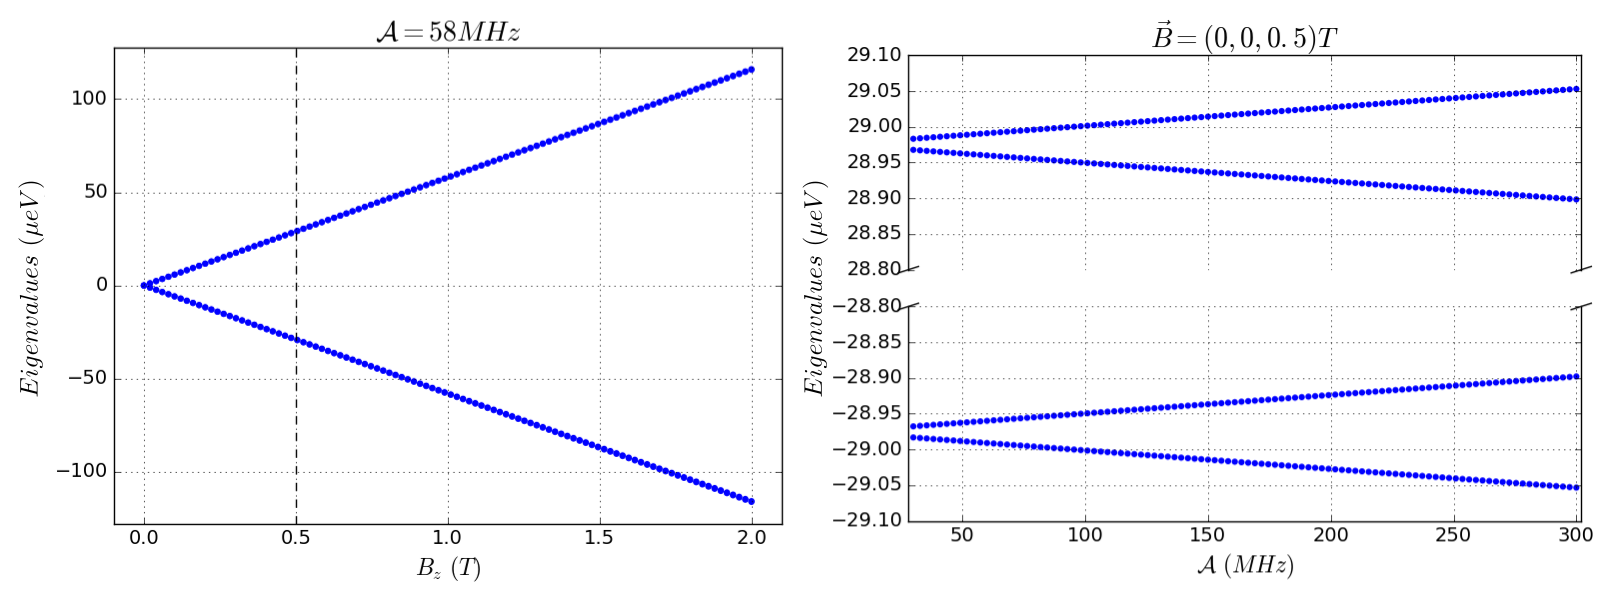
\includegraphics[width=0.9\textwidth]{chapter03/figures/spectrum.png}
\vspace{-5pt}
\caption{Evolution of the eigenvalues of the Hamiltonian \eqref{1qubit} with the magnetic field, $B$, and the hyperfine interaction, $\mathcal{A}$. The dashed line is used to indicate the magnetic field in the second figure}
\label{spectrum}
\end{figure}
\FloatBarrier
%~~~~~~~~~~~~~~~~~~~~~~~~~~~~~~~~~~~~~~~~~~~~~~~~~~~~~~~~~~~%
In figure~\ref{spectrum} we can see that the energy levels are separated in two sets split by the electronic Zeeman splitting (remember that we are neglecting the proton Zeeman coupling here). The splitting within each of these sets is governed by the hyperfine coupling.

But as we said before, the hyperfine coupling and Zeeman coupling for the proton are in the same order of magnitude. When we include the proton Zeeman interaction the big picture is the same: two sets of levels split by the electronic Zeeman. But within each of these two sets there is a difference, depending on the magnitude of the magnetic field and the hyperfine coupling the ordering of the wave functions may change. \red{rephrase}
%~~~~~~~~~~~~~~~~~~~~~~~~~~ FIGURE ~~~~~~~~~~~~~~~~~~~~~~~~~%
\begin{figure}[h!]
\centering
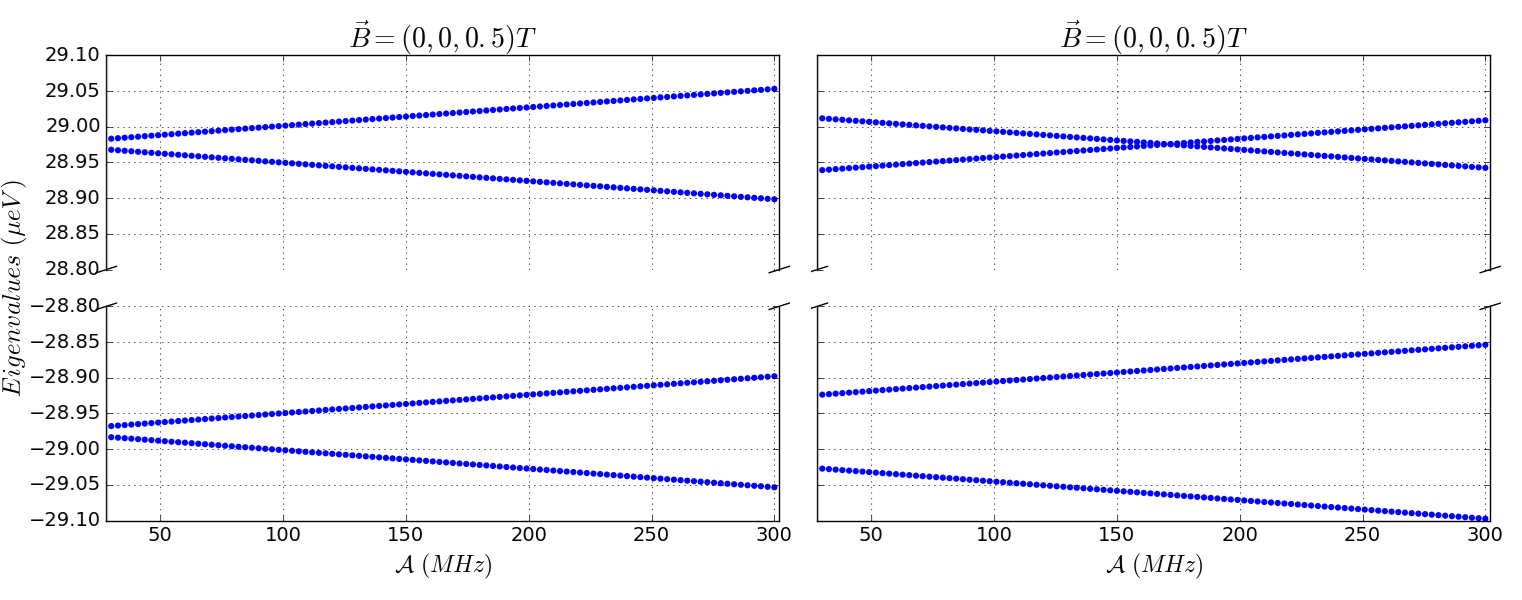
\includegraphics[width=0.9\textwidth]{chapter03/figures/pro_nopro.png}
\vspace{-5pt}
\renewcommand{\figurename}{\footnotesize{\textsc{Figure}}}
\caption{Comparison of the energy levels as a function of the hyperfine coupling. Panel $a)$ neglects the Zeeman term for the proton, in panel $b)$ we use the full Hamiltonian. (Both panels share the $Y$ axis)}
\label{proton}
\end{figure}
\FloatBarrier
%~~~~~~~~~~~~~~~~~~~~~~~~~~~~~~~~~~~~~~~~~~~~~~~~~~~~~~~~~~~%
The level crossing that appears in figure~\ref{proton} represents nothing more than the exchange of the wave functions as it can be seen in the analytical expression~\eqref{eig}. In fact using these expressions we can get the expression for this level crossing:
\begin{equation}
  \mathcal{A}_{\times}=\frac{B}{2}\left(E\pm\sqrt{E^2+4EP}\right)
\end{equation}


To clarify the meaning of this spectrum we make a schematic representation of the eigenfunctions, shown in figure~\ref{levels1Qbit}. The left column in the table represents the wave functions neglecting the proton's Zeeman contribution. The two columns in the right do not neglect the proton's coupling, and show the cases of high magnetic field (or low hyperfine coupling) and low magnetic field (or high hyperfine coupling). It is clear that depending on the relative magnitude of the proton's Zeeman effect and the Hyperfine coupling the order of the wave functions may differ.
%~~~~~~~~~~~~~~~~~~~~~~~~~~ FIGURE ~~~~~~~~~~~~~~~~~~~~~~~~~%
%TODO 0.004 ueV/T add "/T" in the picture. Qbit notation arrow ---> 0/1
\begin{figure}[h!]
\centering
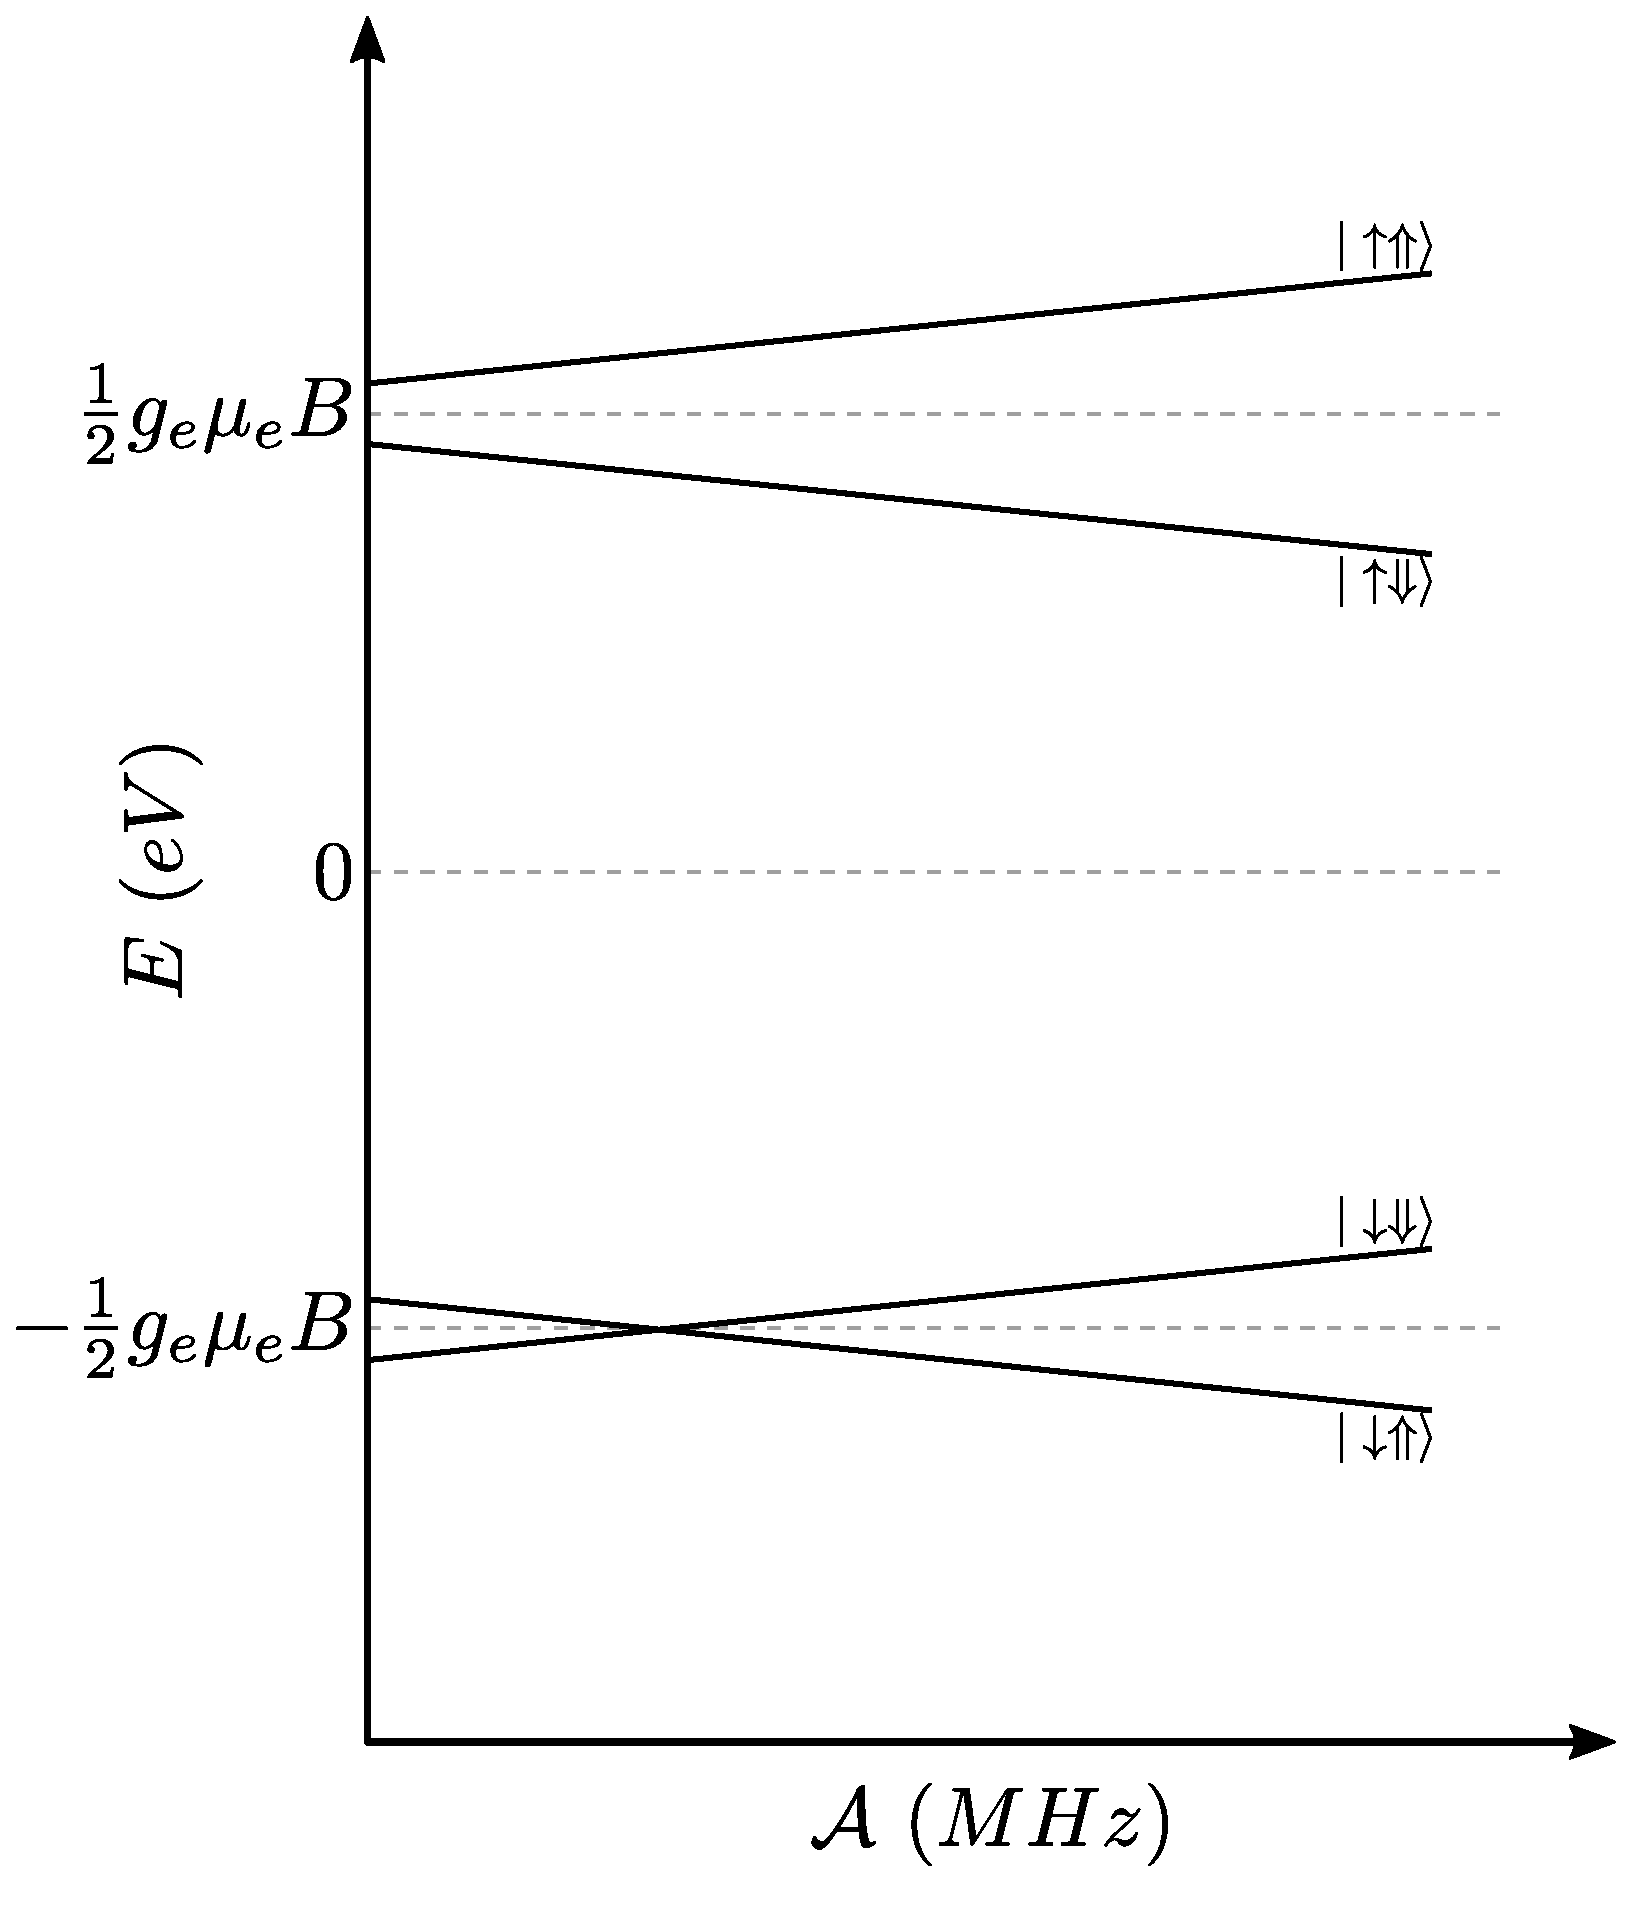
\includegraphics{chapter03/figures/levels1Qbit.pdf} %levels.png}
\vspace{-5pt}
\caption{Sketch of the energy levels for the 1 Qubit Hamiltonian~\eqref{1qubit}. The main splitting among the different states is mainly due to the electronic Zeeman terms. The lowest energy state is determined by the competition between the nuclear Zeeman splitting and the hyperfine interaction.}
% \caption{Schematic representation of the energy levels and its respective wave functions. The states $\ket{\daw\Uaw}$ and $\ket{\uaw\Daw}$ and in fact mixed, but it is negligible (this means that $\ket{\uaw\Daw}\simeq0.9999999\ket{\uaw\Daw}+0.0002672\ket{\daw\Uaw}$). All the possible transitions are specified by $\delta_i$.}
\label{levels1Qbit}
\end{figure}
\FloatBarrier
%~~~~~~~~~~~~~~~~~~~~~~~~~~~~~~~~~~~~~~~~~~~~~~~~~~~~~~~~~~~%
% The states $\ket{\daw\Uaw}$ and $\ket{\uaw\Daw}$ do not in fact appear with weight 1, instead there is a small mixing (less than $0.001\%$).
%
% \red{I think the order of my states is not exactly the same as Morello's. Check}
% Notice that $\delta_1$ and $\delta_2$ will be quite similar ($\SI{50}{\eV/\tesla}$) and $\delta_3$, $\delta_4$ will also be very similar ($\SI{0.05}{\eV/\tesla}$). These frequencies correspond to the energy necessary for flipping respectively the electron spin and the nuclear spin.
%
% \red{Nuclear magnetic resonance and stuff}


\section{The 2-Qubit Hamiltonian}
The general expression for the Hamiltonian of two qubits requires the consideration of Zeeman interactions for each of the electronic and nuclear spins, the hyperfine coupling for each of the qubits, and an exchange term between them. Of course contributions such as  $\mathcal{A}_{1,2}\vec{\sigma}^e_1\vec{\sigma}^e_2$ should also exist, but its contribution would be negligible since the electronic wavefunction decay exponentially. The total Hamiltonian for two qubits, then, reads:
\begin{equation}
  H = H_B +A_1\vec{\sigma}^e_1\cdot\vec{\sigma}^p_1
      +A_2\vec{\sigma}^e_2\cdot\vec{\sigma}^p_2
      +J\vec{\sigma}^e_1\cdot\vec{\sigma}^e_2
\label{ham2Q}
\end{equation}
where $H_B$ contains the Zeeman interactions of each of the electronic and nuclear spins.
\begin{equation}
  H_B = -g_e\mu_e\frac{1}{2}\vec{B}_1\vec{\sigma}^e_1
      -g_p\mu_p\frac{1}{2}\vec{B}_1\vec{\sigma}^p_1
      -g_e\mu_e\frac{1}{2}\vec{B}_2\vec{\sigma}^e_2
      -g_p\mu_p\frac{1}{2}\vec{B}_2\vec{\sigma}^p_2
\label{ham2Q_zeeman}
\end{equation}
To describe two qubits we need again to expand our basis. In particular we will use the notation $\ket{S^z_1I^z_1;S^z_2I^z_2}$. The basis, then, would have 16 elements
\begin{equation}
\begin{split}
 \mathcal{B}_{2Q} =  \left\{\ket{\uaw\Uaw;\uaw\Uaw},\ket{\uaw\Uaw;\uaw\Daw},\ket{\uaw\Uaw;\daw\Uaw},\ket{\uaw\Uaw;\daw\Daw},\right.\\
        \ket{\uaw\Daw;\uaw\Uaw},\ket{\uaw\Daw;\uaw\Daw},\ket{\uaw\Daw;\daw\Uaw},\ket{\uaw\Daw;\daw\Daw},\\
        \ket{\daw\Uaw;\uaw\Uaw},\ket{\daw\Uaw;\uaw\Daw},\ket{\daw\Uaw;\daw\Uaw},\ket{\daw\Uaw;\daw\Daw},\\
 \left.\ket{\daw\Daw;\uaw\Uaw},\ket{\daw\Daw;\uaw\Daw},\ket{\daw\Daw;\daw\Uaw},\ket{\daw\Daw;\daw\Daw} \right\}
\end{split}
\end{equation}
Notice that we are not considering here doubly occupied states such as $\ket{\udaw\Uaw;\quad\Uaw}$ since for now we consider that the two qubits are sufficiently isolated from each other to allow this kind of transitions, in addition to the extra energy that would cost the double occupancy (Hubbard repulsion).

All the operators in eq.~\eqref{ham2Q} have the same dimension as the basis ($16\times16$) and, when diagonalized, they show a spectrum similar to that sketched in fig.~\ref{levels2Qbits}
%~~~~~~~~~~~~~~~~~~~~~~~~~~ FIGURE ~~~~~~~~~~~~~~~~~~~~~~~~~%
\begin{figure}[h!]
\centering
  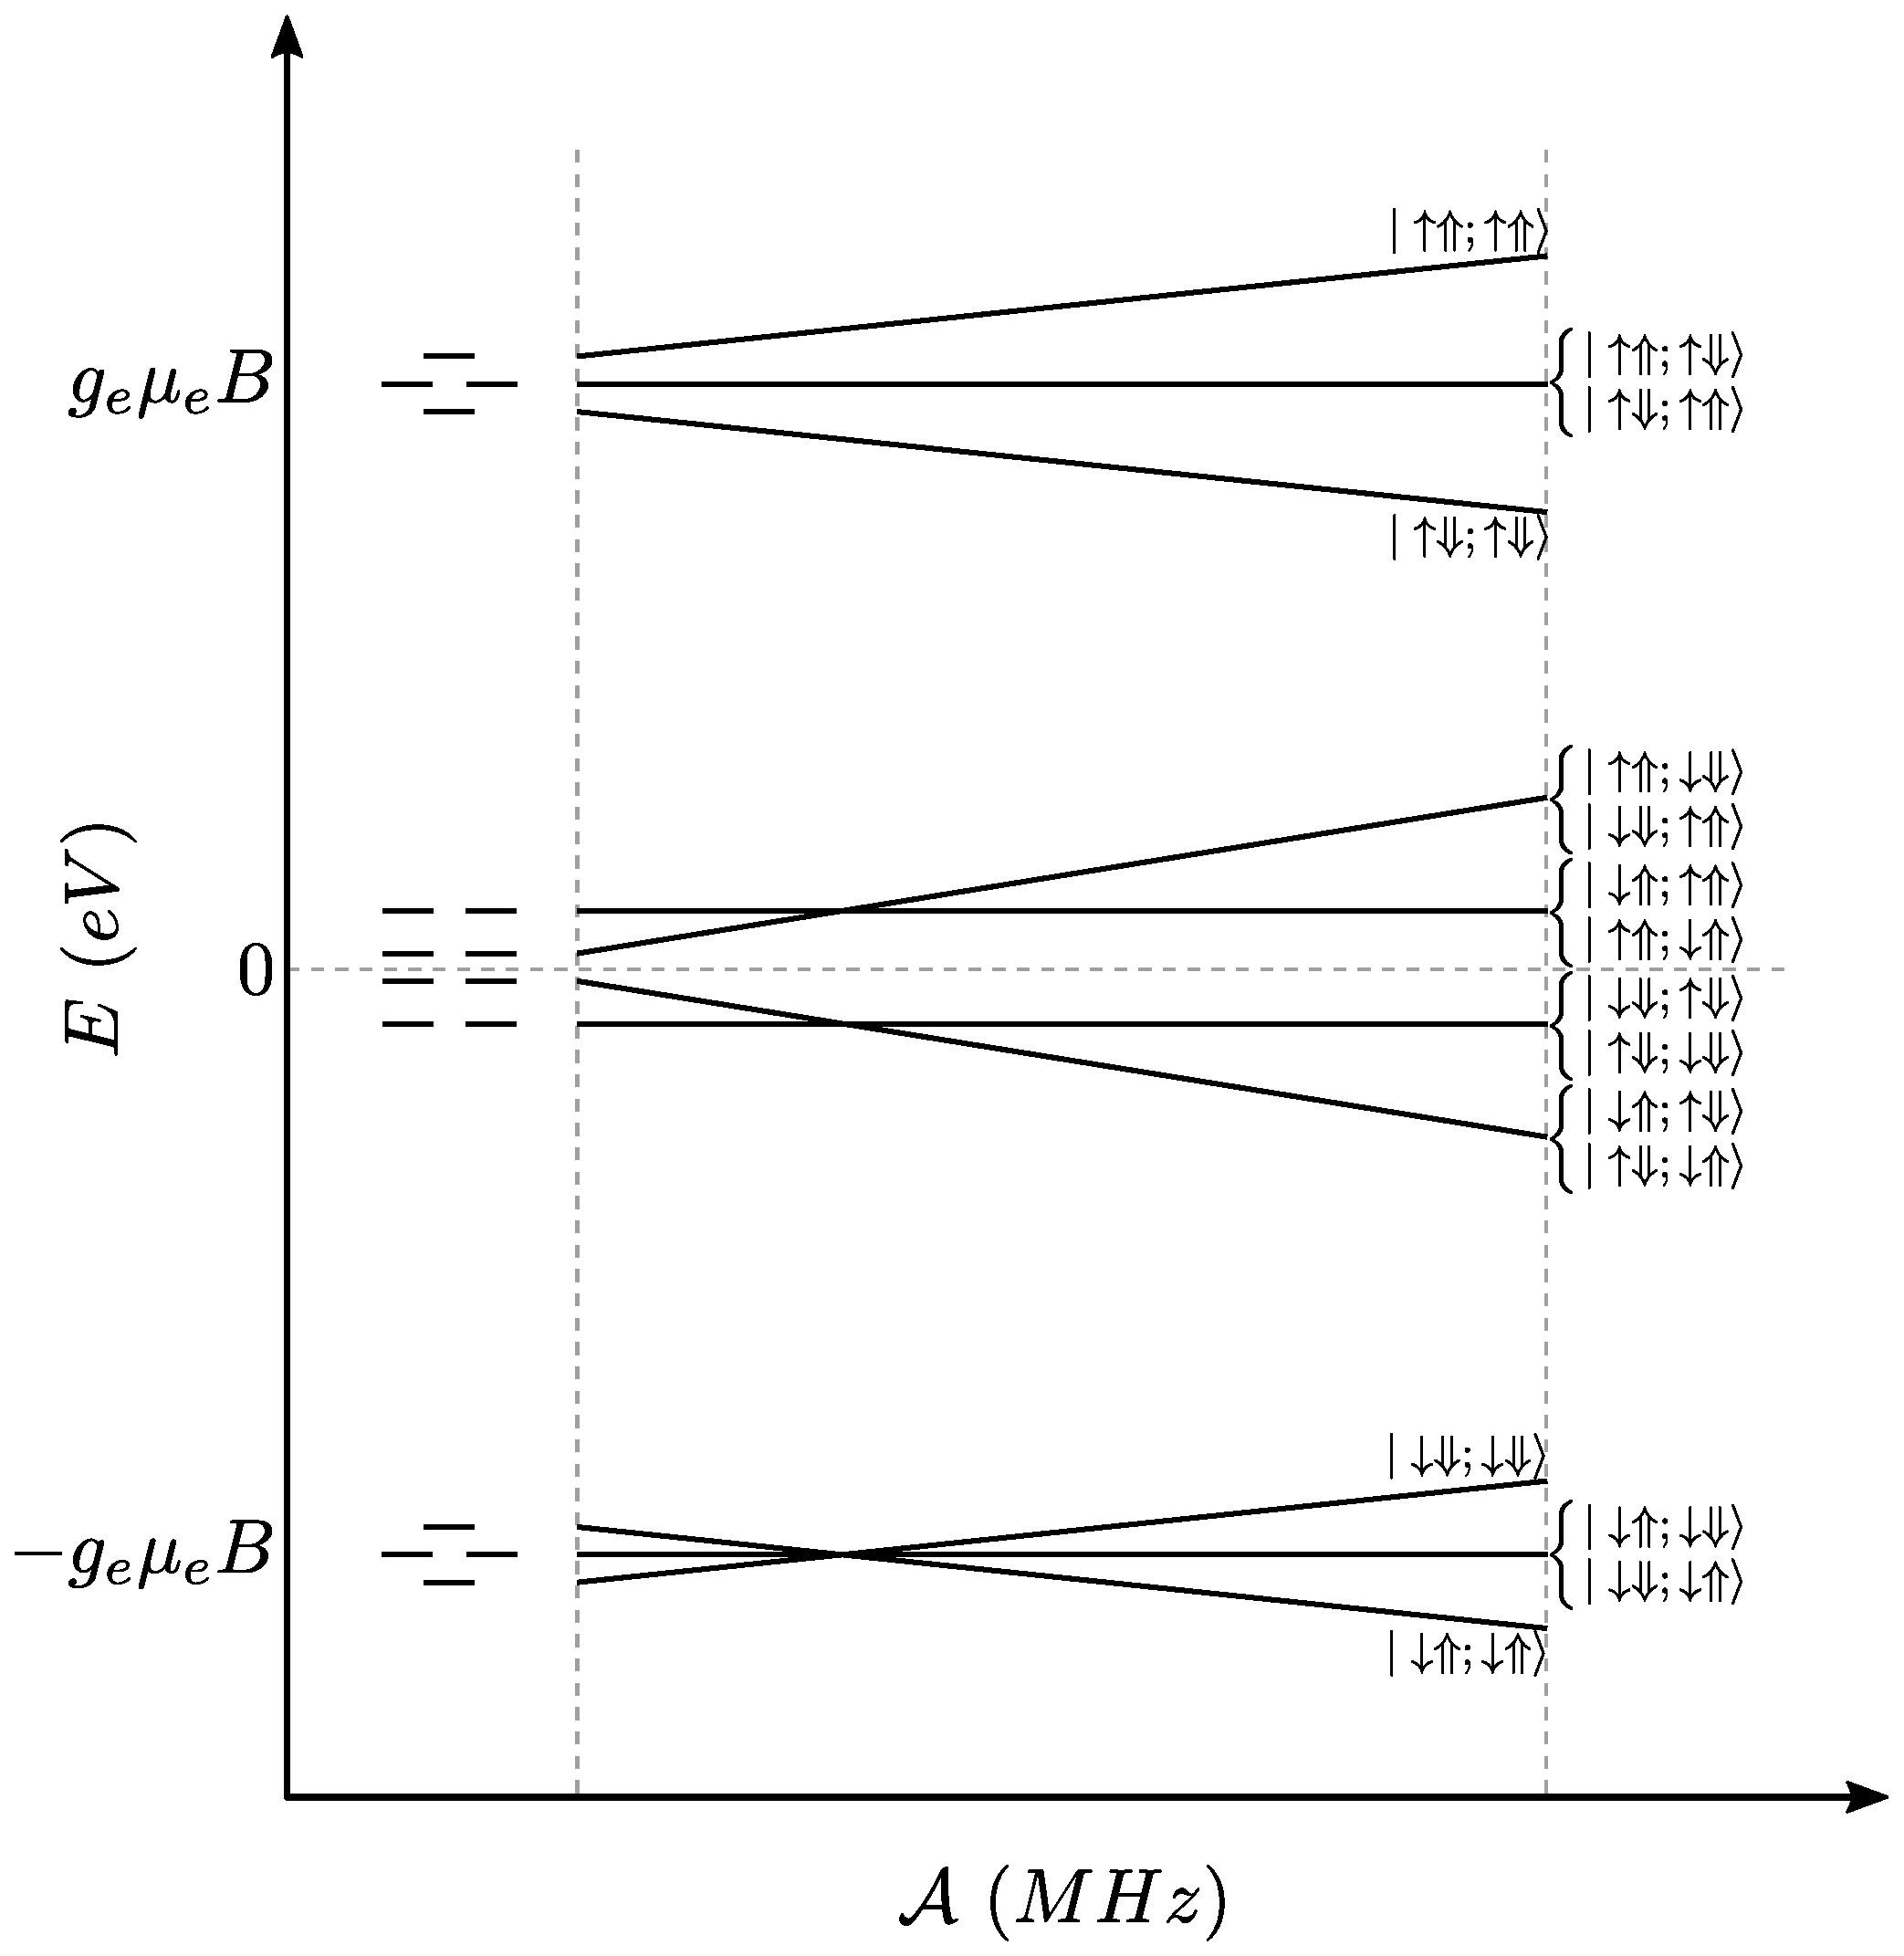
\includegraphics{chapter03/figures/levels2Qbits.pdf}
\vspace{-5pt}
\caption{Sketch of the energy levels of 2 qubits. The spectrum is divided in three sets of levels determined mainly by the electronic Zeeman splitting. The degeneracies and ordering of the states in each of these groups is determined by competition between the nuclear Zeeman and hyperfine couplings as well as the exchange interaction.}
\label{levels2Qbits}
\end{figure}
\FloatBarrier
%~~~~~~~~~~~~~~~~~~~~~~~~~~~~~~~~~~~~~~~~~~~~~~~~~~~~~~~~~~~%
As we  can see, the levels are split in three sets, centered around $E\sim0$ and $E\sim\pm g_e\mu_e B$ respectively. The energy of each of these sets is mainly defined by the electronic spin of each of the two qubits, eq.~\eqref{ham2Q_zeeman} since that is the strongest interaction.
When the electrons of each of the Qubits are parallel (both up or down) the total energy of the system is roughly $E=pm g_e\mu_e B$.
The competition between the Zeeman effect in the nuclear spin and the hyperfine coupling determines which state is the lowest in energy, either $\ket{\Uaw;\Uaw}$ or $\ket{\Daw;\Daw}$. Notice that the solutions in which both electronic spins are parallel and the nuclear spin in each Qubit are different are degenerate in energy.
